
\documentclass[12pt]{beamer}
\usepackage{amsmath}
\usepackage{mathtools}
\usepackage{multimedia}
\usepackage{hyperref}


\usefonttheme{professionalfonts} % using non standard fonts for beamer
\usefonttheme{serif} % default family is serif
%\documentclass[12pt]{beamerthemeSam.sty}
\usepackage{epsf}
%\usepackage{pstricks}
%\usepackage[orientation=portrait,size=A4]{beamerposter}
\geometry{paperwidth=160mm,paperheight=120mm}
%DT favorite definitions
\def\LL{\left\langle}	% left angle bracket
\def\RR{\right\rangle}	% right angle bracket
\def\LP{\left(}		% left parenthesis
\def\RP{\right)}	% right parenthesis
\def\LB{\left\{}	% left curly bracket
\def\RB{\right\}}	% right curly bracket
\def\PAR#1#2{ {{\partial #1}\over{\partial #2}} }
\def\PARTWO#1#2{ {{\partial^2 #1}\over{\partial #2}^2} }
\def\PARTWOMIX#1#2#3{ {{\partial^2 #1}\over{\partial #2 \partial #3}} }

\def\rightpartial{{\overrightarrow\partial}}
\def\leftpartial{{\overleftarrow\partial}}
\def\diffpartial{\buildrel\leftrightarrow\over\partial}

\def\BC{\begin{center}}
\def\EC{\end{center}}
\def\BN{\begin{enumerate}}
\def\EN{\end{enumerate}}
\def\BI{\begin{itemize}}
\def\EI{\end{itemize}}
\def\BE{\begin{displaymath}}
\def\EE{\end{displaymath}}
\def\BEA{\begin{eqnarray*}}
\def\EEA{\end{eqnarray*}}
\def\BNEA{\begin{eqnarray}}
\def\ENEA{\end{eqnarray}}
\def\EL{\nonumber\\}

\newcommand{\etal}{{\it et al.}}
\newcommand{\gbeta}{6/g^2}
\newcommand{\la}[1]{\label{#1}}
\newcommand{\ie}{{\em i.e.\ }}
\newcommand{\eg}{{\em e.\,g.\ }}
\newcommand{\cf}{cf.\ }
\newcommand{\BS}{\bigskip}
\newcommand{\etc}{etc.\ }
\newcommand{\atantwo}{{\rm atan2}}
\newcommand{\Tr}{{\rm Tr}}
\newcommand{\dt}{\Delta t}
\newcommand{\op}{{\cal O}}
\newcommand{\msbar}{{\overline{\rm MS}}}
\def\chpt{\raise0.4ex\hbox{$\chi$}PT}
\def\schpt{S\raise0.4ex\hbox{$\chi$}PT}
\def\MeV{{\rm Me\!V}}
\def\GeV{{\rm Ge\!V}}

%AB: my color definitions
%\definecolor{mygarnet}{rgb}{0.445,0.184,0.215}
%\definecolor{mygold}{rgb}{0.848,0.848,0.098}
%\definecolor{myg2g}{rgb}{0.647,0.316,0.157}
\definecolor{A}{rgb}{1.0,0.3,0.3}
\definecolor{B}{rgb}{0.0,1.0,0.0}
\definecolor{C}{rgb}{1.0,1.0,0.0}
\definecolor{D}{rgb}{0.5,0.5,1.0}
\definecolor{E}{rgb}{0.7,0.7,0.7}
\definecolor{abtitlecolor}{rgb}{1.0,1.0,1.0}
\definecolor{absecondarycolor}{rgb}{0.0,0.416,0.804}
\definecolor{abprimarycolor}{rgb}{1.0,0.686,0.0}
\definecolor{Red}           {rgb}{1,0.4,0.4}
\definecolor{Yellow}           {rgb}{1,1,0.0}
\definecolor{Grey}          {cmyk}{.7,.7,.7,0}
\definecolor{Blue}          {cmyk}{1,1,0,0}
\definecolor{Green}         {cmyk}{1,0,1,0}
\definecolor{Brown}         {cmyk}{0,0.81,1,0.60}
\definecolor{Silver}        {rgb}{0.95,0.9,1.0}
\definecolor{Sky}           {rgb}{0.07,0.0,0.2}
\definecolor{Darkbrown}     {rgb}{0.4,0.3,0.2}
\definecolor{Black}         {rgb}{0.0,0.0,0.0}
\definecolor{40Gray}        {rgb}{0.4,0.4,0.5}
\usetheme{Madrid}


\setbeamercolor{normal text}{fg=Silver,bg=Sky}

%AB: redefinition of beamer colors
%\setbeamercolor{palette tertiary}{fg=white,bg=mygarnet}
%\setbeamercolor{palette secondary}{fg=white,bg=myg2g}
%\setbeamercolor{palette primary}{fg=black,bg=mygold}
\setbeamercolor{title}{fg=abtitlecolor}
\setbeamercolor{frametitle}{fg=abtitlecolor}
\setbeamercolor{palette tertiary}{fg=white,bg=Darkbrown}
\setbeamercolor{palette secondary}{fg=white,bg=absecondarycolor}
\setbeamercolor{palette primary}{fg=white,bg=40Gray}
\setbeamercolor{structure}{fg=abtitlecolor}

\setbeamerfont{section in toc}{series=\bfseries}

%AB: remove navigation icons
\beamertemplatenavigationsymbolsempty
\title[The origin of the Solar System]{
  \textbf {The origin of the Solar System}}

\author [Astronomy 101]{Astronomy 101\\Syracuse University, Fall 2016\\Walter Freeman}

\date{\today}

\begin{document}



\frame{\titlepage}

\frame{
\BC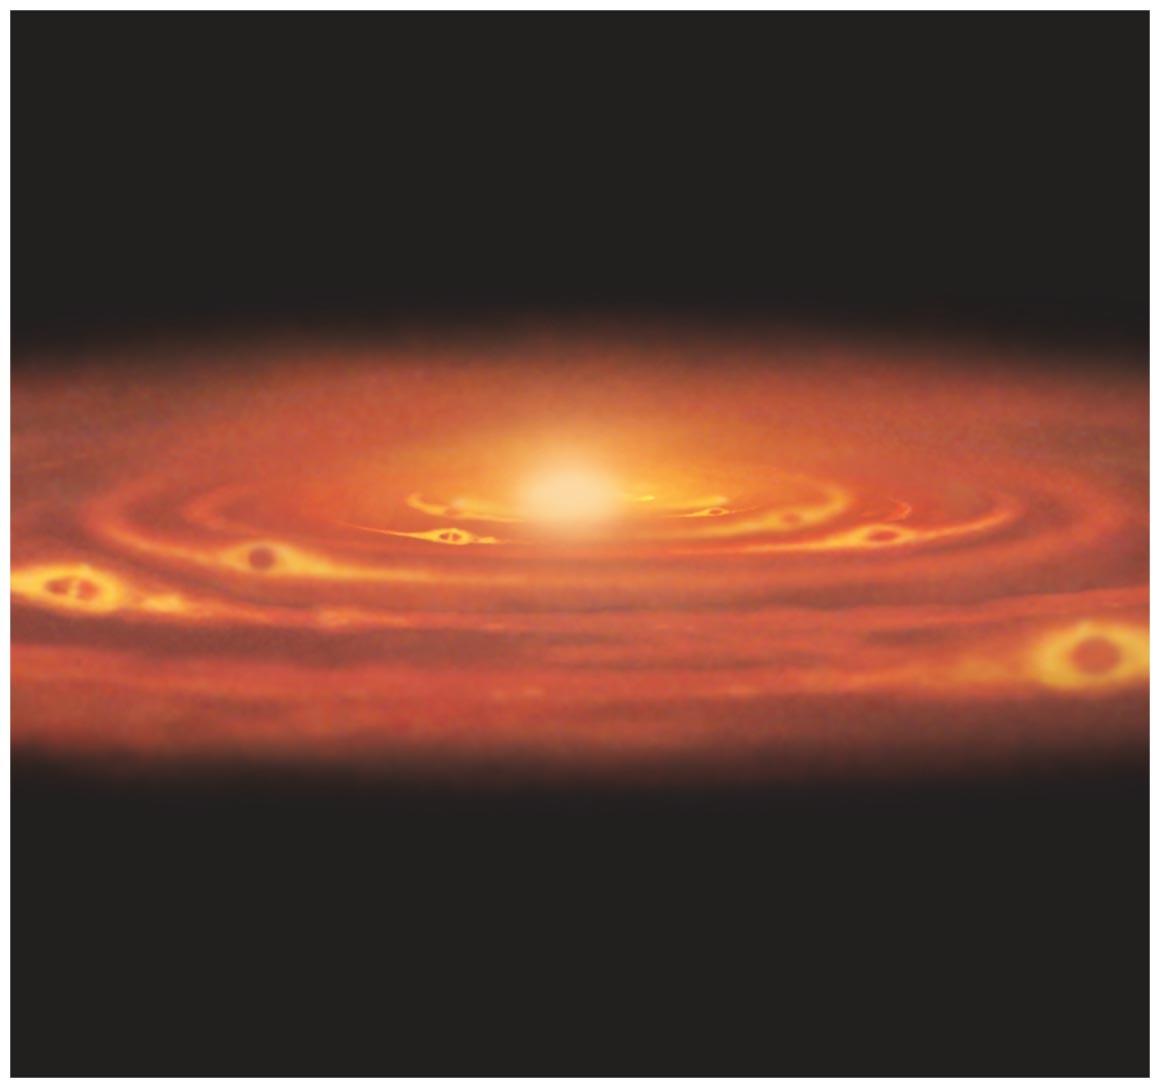
\includegraphics[width=0.7\textwidth]{ss-origin.jpg}\EC
}

\frame{\frametitle{\textbf{Announcements}}
\large
\BI
\item Exam 3 on Tuesday
\BI
\item The exam will cover everything since Exam 2
\item Today's material will not be on the exam (but will be on the final)
\item The bulk of the exam will cover the material on light and the Sun (in the study guide)
\EI
\pause
\item Exam reviews: 
\BI 
\item Friday 9:30-12 (in my office, room 215)
\item Sunday 1-4 (in the physics clinic)
\item Monday (if I get the exam printed in time; I'll send out availability once I know it)
\EI
\item Your second paper is due next Friday
\item I am behind on messages/mail and will catch up Friday morning if I can
\EI
}

\frame{\frametitle{\textbf{A look at the rest of the term}}
\large
We're now in the fourth of our four units: ``where we've come from, and where we're going''. We'll study:

\BS

\large

\pause

\color{Red} Where we've come from:

\BI
\item How the Sun and the solar system formed
\item How the planets formed, the history of Earth, and how we know it
\item The special role of atmospheres -- {\bf the greenhouse effect and climate change}
\item The rest of the Solar System: what else is out there, and what might live there
\EI

\pause
\BS

\color{Green} ... and where we've been and where we'll go:

\BI
\item Travel to the Moon; the current state of spaceflight
\item How we might get to the stars
\item ... and what we might find living there once we do
\EI
}

\frame{\frametitle{\textbf{Your final projects}}
\Large
A few reminders:
\BS
\Large
\BI
\item If you're working in a group, remember you {\it must} submit a proposal to me telling me:
\BI
\item What you're doing, and why you need a group of that size
\item What each person in the group will be doing
\EI
\item You're encouraged to submit proposals for any project idea you would like feedback on, or advice on how to make it connect to astronomy/science better
\pause
\BS
\item People doing visual art or poetry: remember you need to submit a companion piece with your project
\EI
}


\frame{\frametitle{\textbf{Deducing the origin of the Solar System: what do we have to work with?}}
\Large

\BC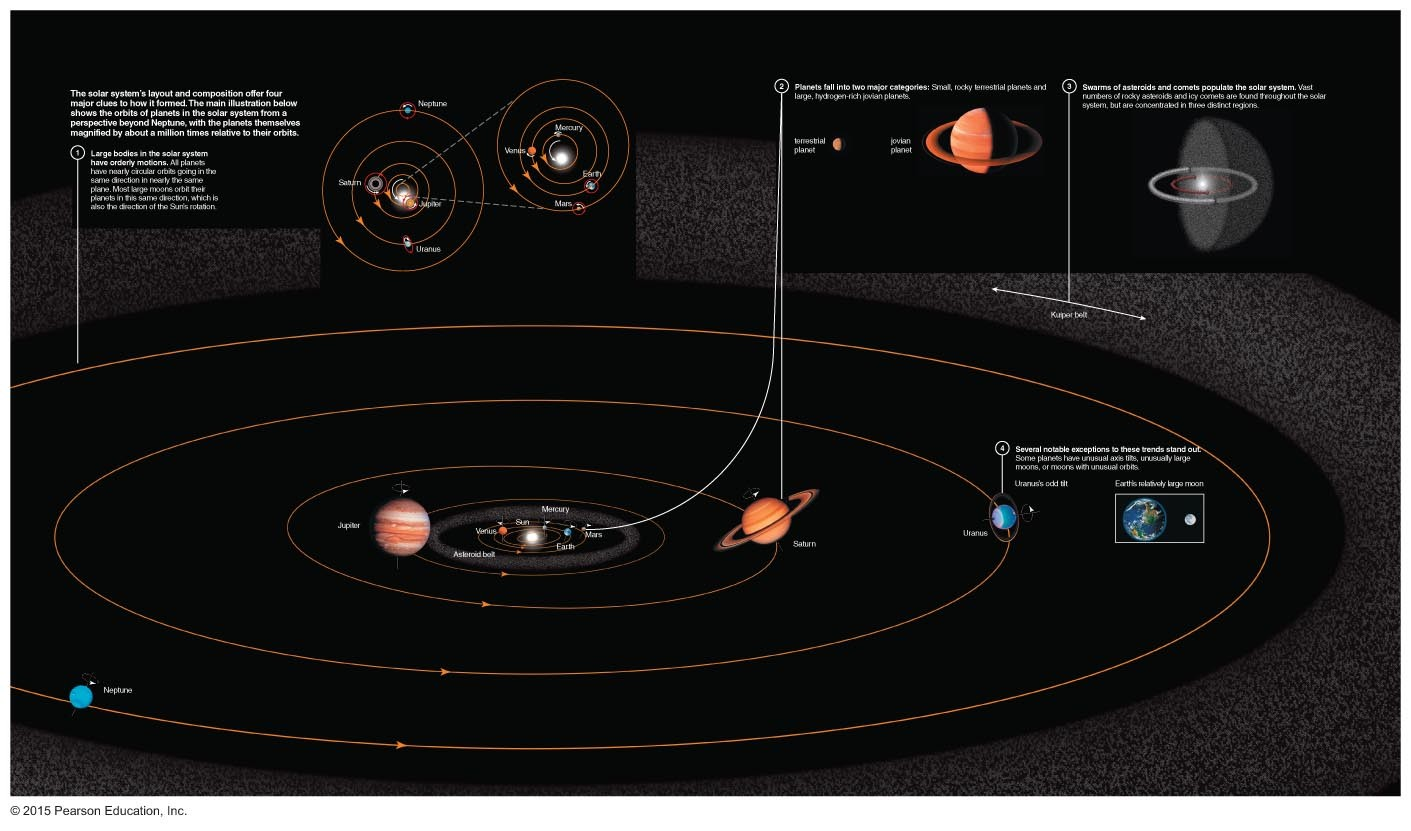
\includegraphics[width=\textwidth]{ss-overview.jpg}\EC

}

\frame{
\Large
\BC
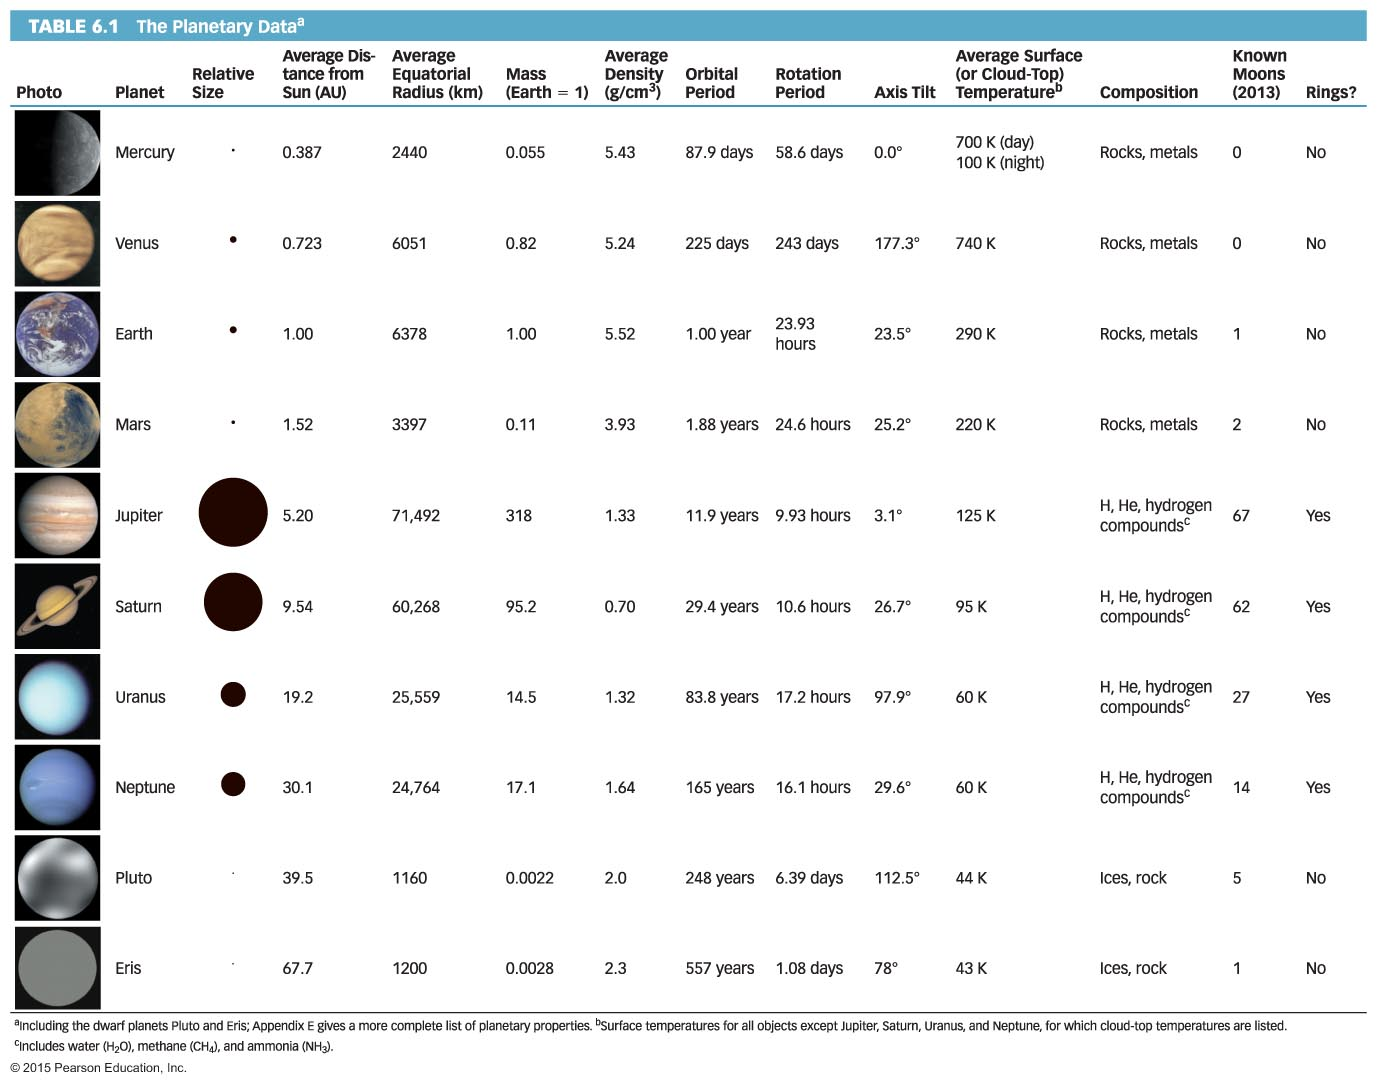
\includegraphics[width=0.9\textwidth]{ss-properties.jpg}
\EC
}


\frame{\frametitle{\textbf{What patterns do we see?}}
\pause

\large
In the inner solar system:
\normalsize
\BI
\item An enormous hydrogen/helium star, with trace elements, at the middle
\item Four small, rocky planets around it, including our own
\BI
\item No large moons here, except Earth's 
\EI
\EI

\pause\BS
\large
In the outer solar system:
\normalsize
\BI
\item Large "gas giant" planets
\item Many hydrogen compounds: water, methane, ammonia
\item Thick atmospheres: hydrogen and helium (mostly)
\item Many moons
\EI

\BS
\large
\pause
Even further out:
\normalsize
\BI
\item The Kuiper belt:
\BI
\item Lots of small icy bodies (Pluto and Eris among them)
\item Orbit roughly along the plane of the solar system
\EI
\item The Oort cloud:
\BI
\item Contains trillions of comets
\item More distant than the Kuiper belt
\item Roughly spherical
\EI
\EI
}

\frame{\frametitle{\textbf{Organized motion}}

\Large
All the planets orbit in the same plane in nearly circular orbits going in the same direction. Most rotate in the same direction, too. Why might this be?

\bigskip
\bigskip
\bigskip

\color{A}A: Long ago all the planets were in contact with each other \\\medskip
\color{B}B: Kepler's laws require this \\\medskip
\color{C}C: Over time the Sun's gravity pulls the planets into circular orbits and synchronizes their rotation \\\medskip
\color{D}D: The planets all formed from the same chunk of the Sun that was knocked off billions of years ago \\\medskip
\color{E}E: It's just a coincidence

}

\frame{\frametitle{\textbf{Organized motion}}
The Solar System formed out of a cloud of gas that collapsed under its own gravity.

\BC
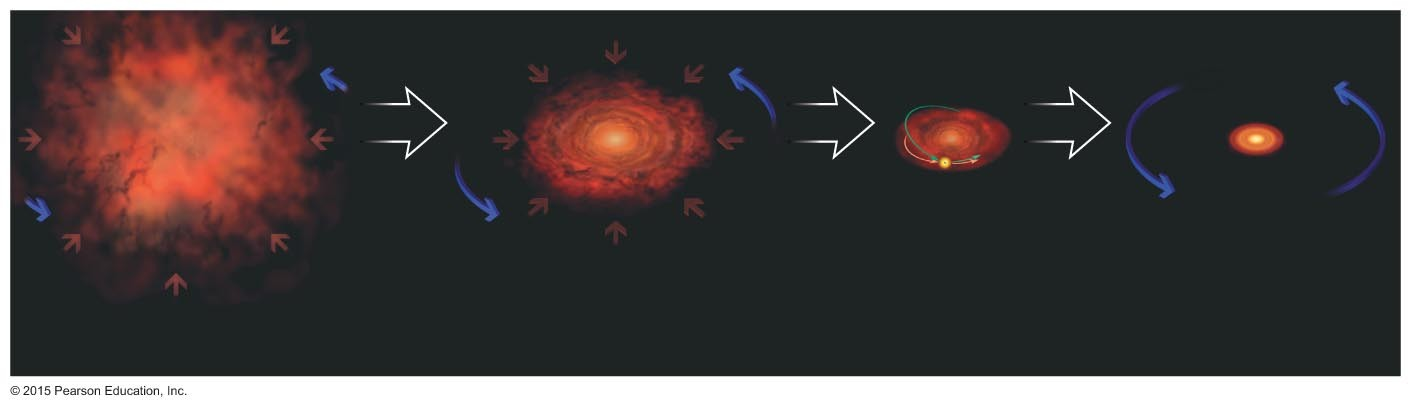
\includegraphics[width=\textwidth]{nebula-history.jpg}
\EC
}

\frame{

\BC
\Large

What should happen to its rotation as it shrinks?
\EC
\BS
\BS

\color{A}A: It should slow down, because of friction between the gas \\\medskip
\color{B}B: It should slow down, because of the mutual gravitation between the different pieces \\\medskip
\color{C}C: It should speed up, because spinning things that shrink in size spin faster \\\medskip
\color{D}D: It shouldn't change, because nothing is applying a twisting force to it \\\medskip
\color{E}E: It should slow down, because spinning things that shrink in size spin slower
}

\frame{\frametitle{\textbf{Angular momentum}}

\large

Physics is very fond of conservation laws. We already met one: the conservation of energy.

\BS

Another conserved quantity is {\it angular momentum}. The angular momentum of an object is the product of:

\BI
\item Its mass, multiplied by
\pause
\item ... how quickly it spins, multiplied by ...
\pause
\item ... {\color{Red}how far its mass is from its center}.
\EI

Since angular momentum is conserved, it doesn't change unless an external agent applies a twist to something.

\BS

We can also get to Kepler's second law from here!
}

\frame{

\large

The primordial universe contained only hydrogen and helium. Where do you think the heavier elements (``metals'') came from?

\BS
\BS

\color{A}A: They're needed for life, and our solar system is special; they aren't found in other solar systems \\\medskip
\color{B}B: All stars contain small amounts of metals \\\medskip
\color{C}C: Nuclear fusion in the Sun builds them out of hydrogen and helium \\\medskip
\color{D}D: Nuclear fusion in earlier stars forges heavier elements out of lighter ones; those stars have since exploded

}


\frame{\frametitle{\bf A spinning cloud of gas}
\BC
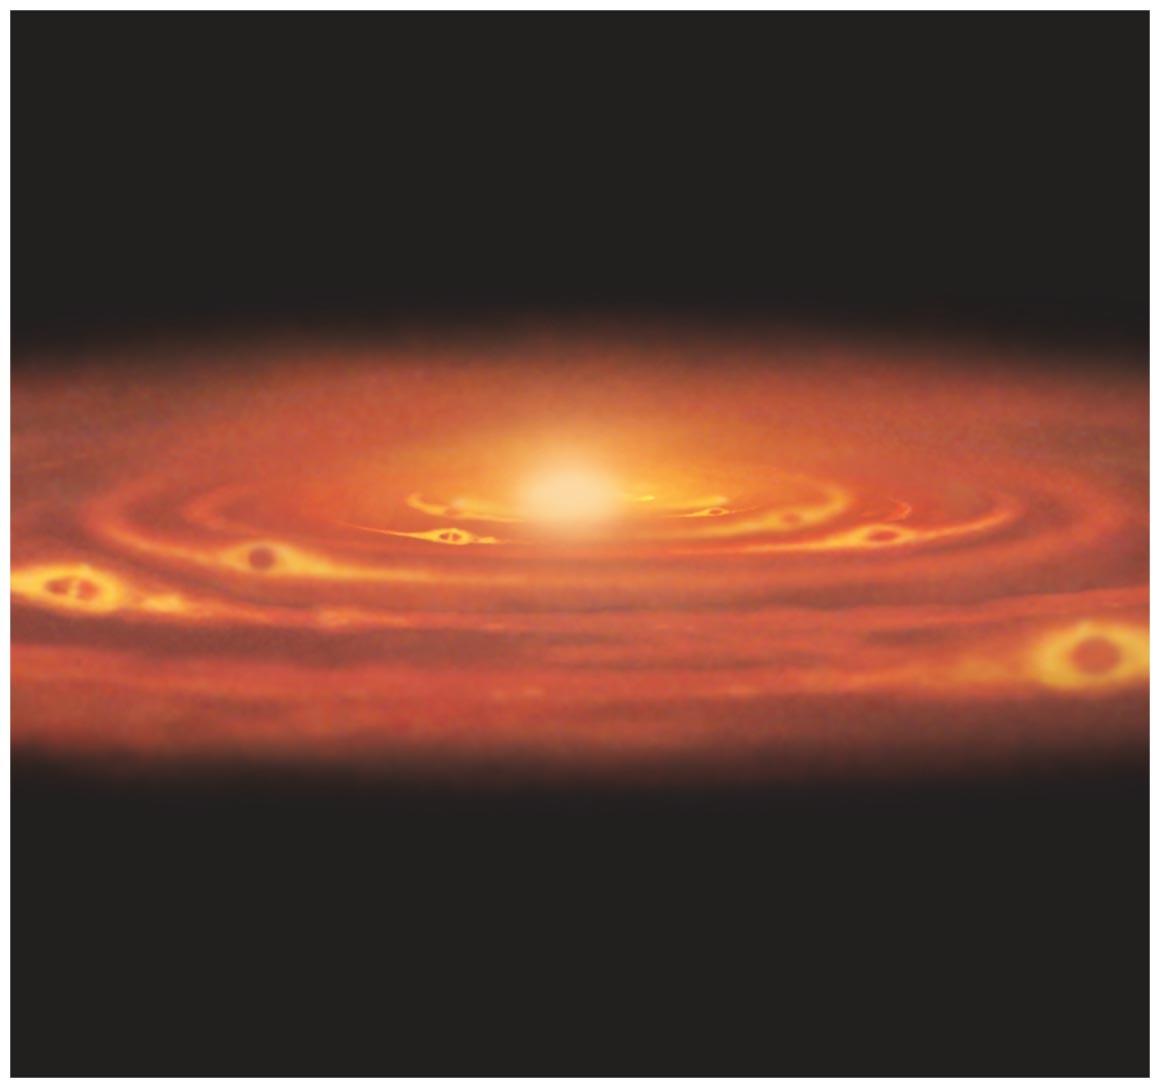
\includegraphics[width=0.5\textwidth]{ss-origin.jpg}
\EC

\pause

At the center, where the gas is most dense, hydrogen accumulated, until gravity was strong enough to kindle fusion. The Sun was born.
}

\frame{\frametitle{\bf What about the planets?}
\BC
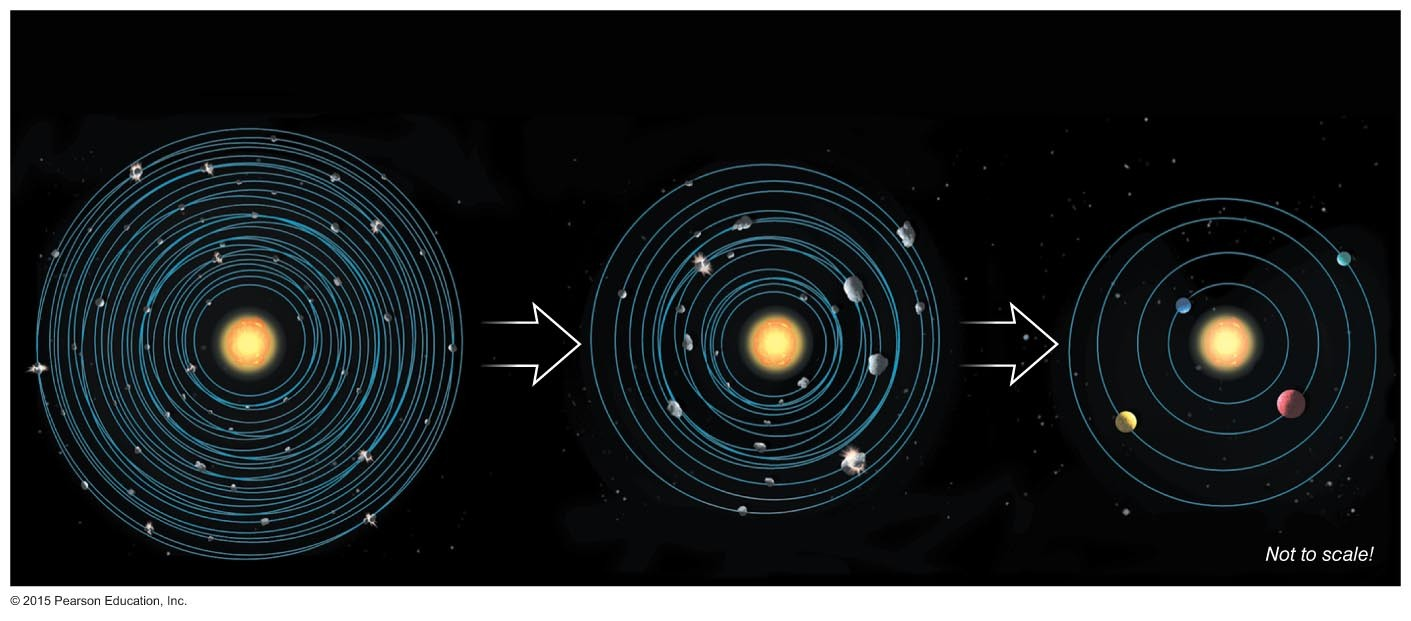
\includegraphics[width=0.8\textwidth]{planetesimals.jpg}
\EC

\pause

The planets condensed out of bits of dust that first formed by static electricity, then as they grew larger, by gravity.

\BS

The gas giants were large enough that they accreted a great deal of gas as well.
}

\frame{

\BC
\Huge
Complete {\it Lecture Tutorials} pp. 111-112.

\small\BS\BS

We will have some time for Exam 3 review after this.

\EC
}


\frame{\frametitle{\bf Why are there different sorts of planets?}
The primordial nebula contained different constituents which condense at different temperatures:

\BS
\BI
\item Hydrogen and helium: never condense in the nebula (98\%)
\item Hydrogen compounds (water, methane, ammonia): condense at less than 150K (1.4\%)
\item Rocks: condense at 500-1300K (0.4\%)
\item Metals: condense at 1000-1600K (0.2\%)
\EI

Further out it is colder, and those hydrogen compounds could condense to form the jovian (``Jupiter-like'') planets.

}


\frame{\frametitle{\bf So here we are...}
\BC
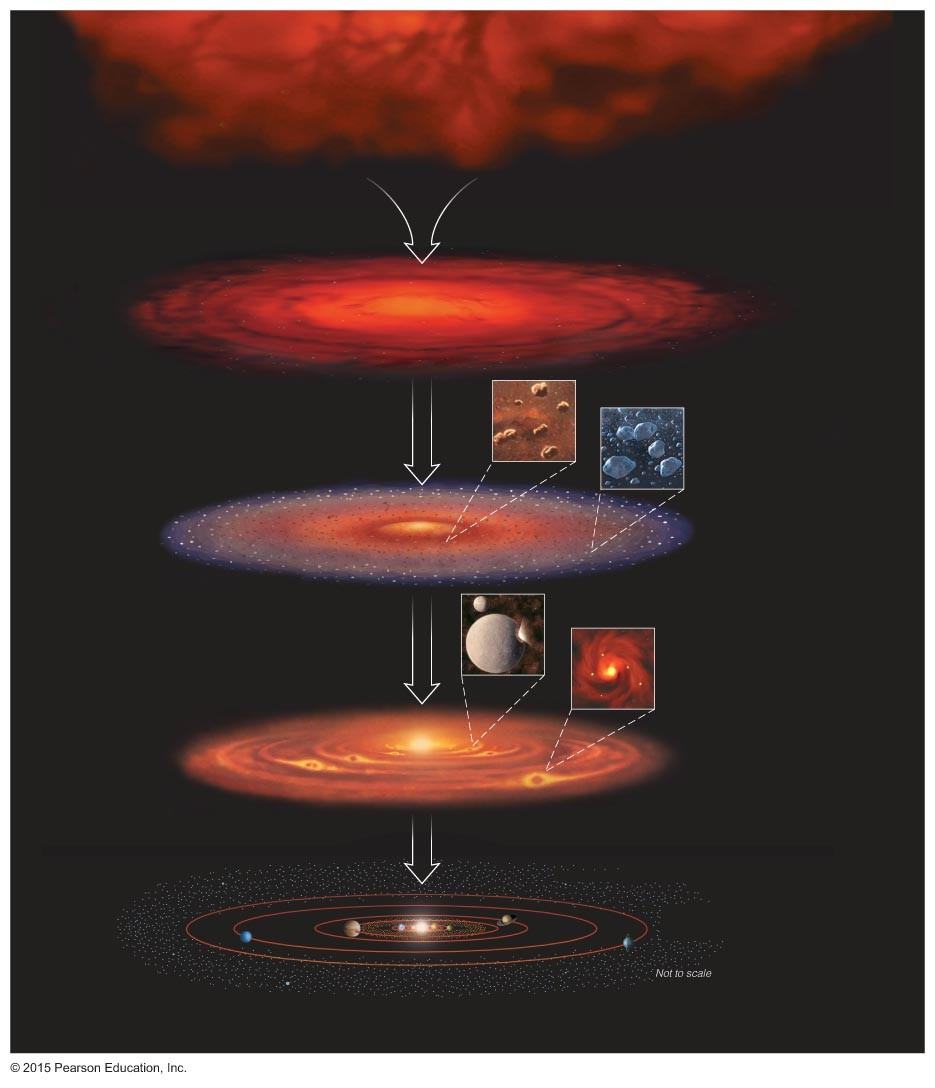
\includegraphics[width=0.5\textwidth]{ss-full-history.jpg}
\EC
}



\end{document}

